\chapter{Data preparation} \label{ch:data_preparation}

The "wicked" nature of transportation and land use interaction introduced in chapter~\ref{ch:background} dictates the need to iteratively "re-solve" transportation and land use planning problems instead of focusing on finding some single "optimal solution".
This approach resembles the methodologies typically employed for data science projects, where the sequence of steps is iterated over, producing a more meaningful solution on each new iteration of the cycle, as defined by such process models as CRISP-DM\cite{Shearer2000}.
Similarly, data preparation can be followed in a linear manner, but is very likely to be iterative in nature\cite{Brownlee2013}.

\vspace{5mm}

Data preparation plays a critical role in research projects:

\begin{itemize}
    \item it is a prerequisite for any meaningful analysis
    \item data quality and the amount of useful information that it contains can determine the success of application of machine learning algorithms\cite{RaschkaMirjalili2017}
    \item it is often required to allow the introduction of constraints necessary for implementation of RDBMS
\end{itemize}

\vspace{5mm}

To facilitate easy modification and replication of the data preparation process for data sources related to the GTHA housing market, a streamlined data preparation workflow using Python via a series of jupyter notebooks has been established as a part of this master's thesis.
It accomplishes three main objectives:
\begin{itemize}
    \item clean Teranet dataset and correct its records for consistency
    \item introduce new keys that allow efficient joining of other data sources such as Census or TTS, while maintaining the integrity of spatial and temporal relationships that were discussed in chapter~\ref{ch:spatial_and_temporal_relationships}
    \item engineer new features that can be used by the machine learning algorithm along with the features from the joined datasets to classify land use, which will be discussed in chapter~\ref{ch:ml_workflow}
\end{itemize}

This chapter introduces the concepts of ''Tidy Data'' and database normalization and outlines the standardized data preparation workflow for all data sources related to the GTHA housing market.

\section{Tidy data and database normalization} \label{sec:db_norm_tidy_data}

Hadley Wickham in his paper ''Tidy Data''\cite{Wickham2014} formalized the way how a shape of the data can be described and what goal should be pursued when formatting data.
The tidy data standard is closely related to Edgar F. Codd's relational algebra and has been designed to facilitate initial exploration and analysis of the data, and to simplify the development of data analysis tools that work well together.
As an integral part of his relational model, Codd\cite{Codd1990} proposed a process of database normalization, or restructuring of a relational database in accordance with a series of so-called normal forms in order to reduce data redundancy and improve data integrity.
Normalization entails organizing the columns (attributes) and tables (relations) of a database to ensure that their dependencies are properly enforced by database integrity constraints.
The principles of ''tidy data'' essentially reformulate Codd's ideas in statistical language.

According to Wickham\cite{Wickham2014}, ''tidy data'' is a standard way of mapping the meaning of a dataset to its structure.
A dataset is ''messy'' or ''tidy'' depending on how rows, columns and tables are matched up with observations, variables and types.

\vspace{5mm}

In ''tidy data'':
\begin{enumerate}
    \item Each variable forms a column.
    \item Each observation forms a row.
    \item Each type of observational unit forms a table.
\end{enumerate}

This is Codd's 3rd normal form\cite{Codd1990}, but with the constraints framed in statistical language, and the focus put on a single dataset rather than the many connected datasets common in relational databases.
''Messy data'' is any other arrangement of the data.

\vspace{5mm}

The structure of Teranet's dataset conforms with the ''Tidy data'' format.
Contrary to Teranet, tables with combined selected Census and TTS variables have variables for different Census and TTS years recorded as columns.
This needs to be addressed by ''melting'' these tables and introducing a new attribute 'year' to be used as a part of a composite foreign key when joining with Teranet records.

\vspace{5mm}

Census and TTS tables were ''melted'' into the ''tidy data'' format:
\begin{itemize}
    \item each Census / TTS variable now forms a single column
    \item each value of a variable is indexed by a composite primary key constituting of spatial identifier and year of the survey
    \item spatial identifiers are 'DAUID' or 'TAZ\_O' (unique identifier for Dissemination Areas or Traffic Analysis Zones introduced in section~\ref{sec:spatial_relationships})
\end{itemize}

Introduction of new foreign keys is described in the following section.

\section{Introduction of new keys and attributes via spatial and temporal relationships} \label{sec:introduction_of_new_keys}

As no combination of columns constitutes a candidate key for Teranet records (unique identifier to be used in RDBMS), a surrogate key (artificial unique identifier for RDBMS) is added to the Teranet dataset via a new attribute 'transaction\_id'.
Thus, Teranet's dataset fits into a normalized database, with the new attribute 'transaction\_id' as its primary key.
As was discussed in section~\ref{sec:db_norm_tidy_data}, the ''melted'' Census and TTS tables have composite primary keys consisting of a unique spatial identifier ('DAUID' or 'TAZ\_O', respectively) and the year of the survey.

To implement the spatial and temporal relationships between the data sources discussed in chapter~\ref{ch:spatial_and_temporal_relationships}, a number of new foreign keys needed to be introduced to Teranet records.
The new foreign keys either represent spatial identifiers (such as 'dauid' or 'taz\_o', corresponding to DA or TAZ within which a Teranet record is located), or an attribute identifying the year of the Census or TTS survey to which this Teranet record can be joined.
Foreign keys representing spatial identifiers are added through a series of spatial joins while foreign keys identifying temporal spans are produced based on temporal relationships established in section~\ref{sec:termporal_relationships_between_datasets}.

\vspace{5mm}

New spatial identifiers were introduced to each Teranet record via a series of spatial joins:
\begin{enumerate}
    \item 9'039'241 Teranet points were joined with 9'182 polygons of Dissemination Areas (DAs) for GTHA used by Census variables
    \begin{itemize}
        \item Teranet records with coordinates falling outside of GTHA boundary were filtered out
        \item From the original 9'039'241 records, 6'803'691 remained in the dataset
        \item New foreign keys 'dauid', 'csduid' and attribute 'csdname' were added to each Teranet record
    \end{itemize}
    \item 6,803,691 Teranet points were joined with 1,716 polygons of Traffic Analysis Zones (TAZ) used by TTS variables
    \begin{itemize}
        \item New foreign key 'taz\_o' was added to each Teranet record
    \end{itemize}
    \item 6,803,691 Teranet points were joined with 525 polygons of Forward Sortation Areas (FSA) and 555,668 polygons of postal geography from DMTI's Platinum Postal Geography Suite
    \begin{itemize}
        \item New foreign keys 'fsa' and 'pca\_id' and attribute 'postal\_code\_dmti' were added to each Teranet record
        \item These keys are not currently used for joining any variables, but were added to expand the potential for relating datasets
    \end{itemize}
    \item 6,803,691 Teranet points were joined with 1,664,862 polygons of parcel-level detailed land use provided by the Department of Geography
    \begin{itemize}
        \item New foreign keys 'pin\_lu', 'landuse' and 'prop\_code' were added to each Teranet record
        \item Foreign keys 'landuse' and 'prop\_code' are codes that can be converted to land use categories that were used by the Department of Geography for GTA and Hamilton, respectively
        \item For records from Hamilton, 'prop\_code' was converted to categories used by GTA land use and reassigned to 'landuse', bringing GTA and Hamilton records to a single system of land use categories
    \end{itemize}
    \item Subsets of Teranet points were joined with corresponding yearly polygons of parcel-level land use from DMTI
    \begin{itemize}
        \item New attribute 'dmti\_lu' was added to each Teranet record
    \end{itemize}
\end{enumerate}

\begin{figure}[hbt!]
    \centering
    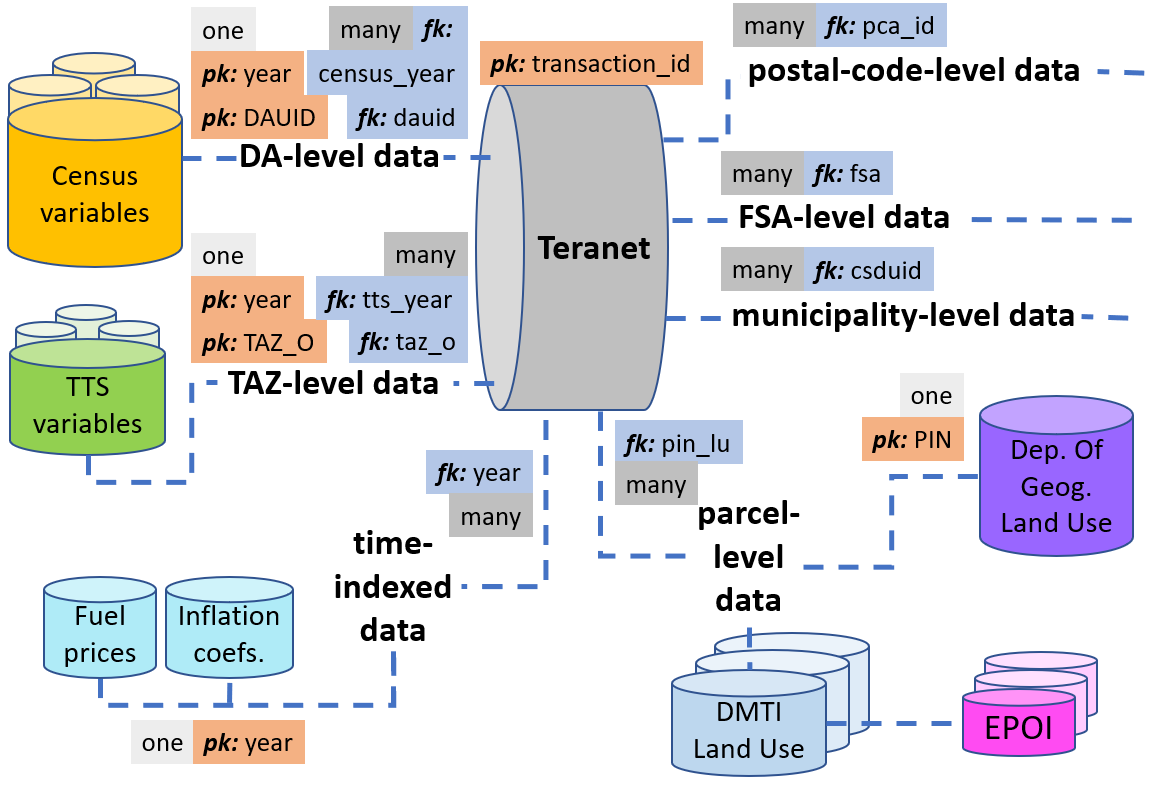
\includegraphics[width=1\linewidth,trim=0 0 0 0,clip]{data_relations.png}
    \caption{Relationships between datasets introduced during data preparation were then used to set up referential integrity constraints of the new PostgreSQL database for GTHA housing market data.}
    \label{fig:data_relations}
\end{figure}

Foreign keys representing temporal identifiers are generated from the registration date of each Teranet record, matching each year of Teranet records to a corresponding 5-year span covered by a Census or TTS survey, as was discussed in section~\ref{sec:termporal_relationships_between_datasets}.
Diagram of relationships between datasets and their primary and foreign keys is presented on figure~\ref{fig:data_relations}

Following the steps described above ensures that the integrity of spatial and temporal relationships is maintained when combining attributes from different data sources at Teranet transaction level.
For example, Teranet records from 2007 would be spatially joined with DMTI land use data from 2007, and are matched by their attributes 'census\_year' and 'tts\_year' to Census and TTS variables from 2006 Census and TTS surveys.
Census and TTS variables can be joined by appropriate 'dauid' and 'taz\_o' (composite foreign keys are used when joining), and thus all data sources can be spatially and temporally aligned at the level of Teranet transactions.

Relationships introduced via the operations described in this section formulate referential integrity constraints that have been used to set up a PostgreSQL database of GTHA housing market data.

\section{Outliers} \label{sec:outliers}

Outliers present an issue for machine learning as they lead to difficulties in visualizing data and, more importantly, can degrade the predictive performance of an algorithm.
In addition, outliers, if left unscaled, can significantly slow down or even prevent the convergence of many gradient-based algorithms, such as Logistic Regression\cite{Scikit-learndevelopers2019b}.
However, an exact definition of what constitutes on outlier within a given dataset presents a challenge in itself, since it depends on hidden assumptions regarding the data structure and the applied detection method\cite{Ben-Gal2005}.
As defined by Hawkins, an outlier is an observation that deviates so much from other observations as to arouse suspicion that it was generated by a different mechanism\cite{Hawkins1980}.

\begin{figure}[ht]
    \centering
    \begin{subfigure}{\linewidth}
        \centering
        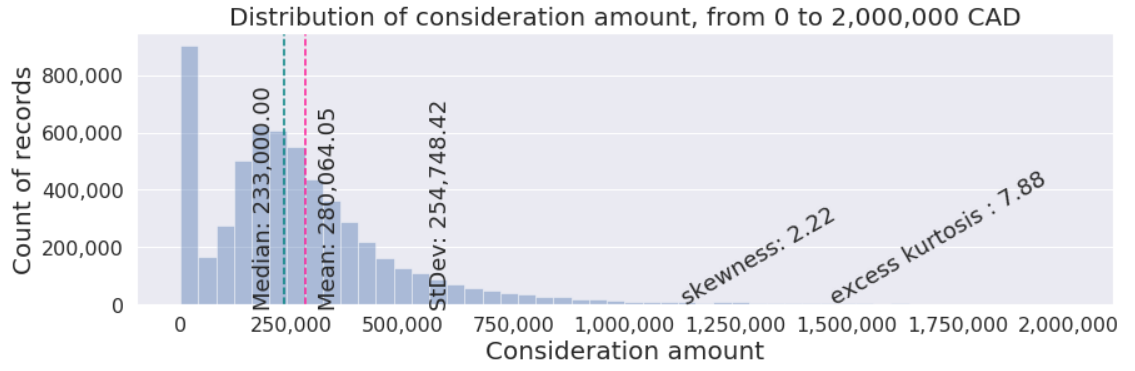
\includegraphics[width=.95\linewidth]{price_dist_raw.png}
        \caption{From 0 to 2'000'000 CAD}
    \end{subfigure}

    \begin{subfigure}{\linewidth}
        \centering
        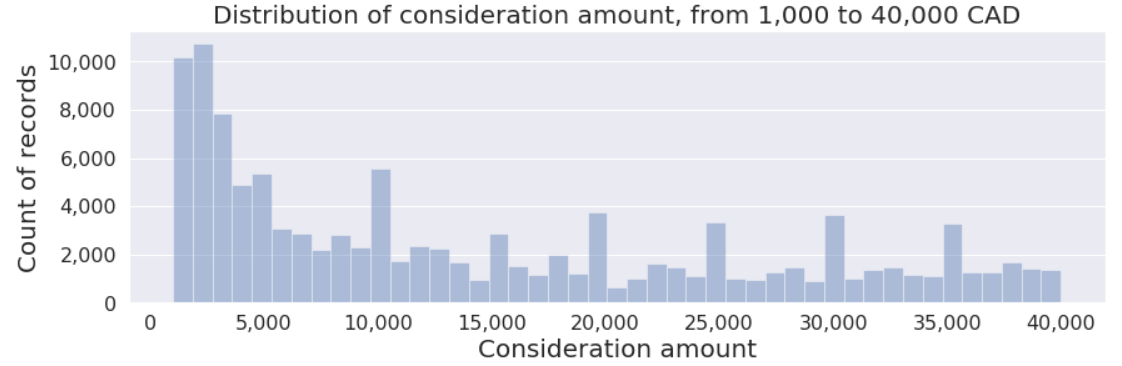
\includegraphics[width=.95\linewidth]{price_dist_zoom.png}
        \caption{From 0 to 40'000 CAD}
    \end{subfigure}
    \caption{Outliers at the bottom end of the price distribution most likely represent gift transactions.
    Since no clear break can be identified, 10'000 CAD was used as the bottom cut-off threshold for consideration amount to filter Teranet records.}
    \label{fig:bottom_outliers}
\end{figure}

In terms of transaction price distribution, outliers at both the high and the low end are present in Teranet's dataset:
\begin{itemize}
    \item There is a high number of transactions with very low consideration amounts (starting from a few dollars) that most likely represent transactions recording gifts of property, where some symbolic consideration amount has been used.
    A large spike can be seen on the low end of the distribution of consideration amount presented on figure~\ref{fig:bottom_outliers}; this spike corresponds to gift transactions with symbolic prices.
    \item At the same time, since the dataset includes all types of property transactions, some records have very high values (ranging in the hundreds of millions and billions of dollars) that most likely correspond to transactions recording sales of large commercial and industrial properties or whole residential buildings.
\end{itemize}

Since low outliers represent transactions that are not useful for analysis, they were removed from the dataset.
However, there seems to be no way to establish what constitutes a reasonable bottom cut-off threshold, as there is no criteria available to determine a gift transaction and there is no distinct break in the price distribution.
Since there seems to be en exceptionally large spike of transactions with consideration amount under 10'000 CAD, they were considered to be low outliers and were removed from Teranet's dataset, further reducing the number of records from 6,803,691 to 5,188,513.

In case of outliers at the high end of price distribution, they most likely correspond to transactions of expensive commercial and industrial property or whole residential buildings.
Since these transactions are useful for research questions concerning commercial and industrial property, they were left in the dataset and instead have been marked with special new attributes ''outlier'' using different criteria.
Since, again, there was no clear criteria available as to what would constitute an outlier, instead of using a single criterion, seven different Boolean variables were added describing whether a record belongs to outliers according to a particular condition or not.
For example, feature 'outlier\_y\_10' is a Boolean variable capturing if the price of a record, corrected for inflation, is over 10 times greater than the median price of all records for the corresponding year.
Table~\ref{tab:outliers} presents the outlier categories that were used and the count of records that each of them marked to belong to outliers.

\begin{table}[h!]
    \centering
    \begin{tabular}{|| c | c ||}
        \hline
        Category & Count of records \\
        \hline
        \hline
        outlier\_y\_3 & 251,537 \\
        \hline
        outlier\_y\_5 & 137,814 \\
        \hline
        outlier\_y\_10 & 84,260 \\
        \hline
        outlier\_y\_20 & 53,866 \\
        \hline
        outlier\_xy\_2 & 160,662 \\
        \hline
        outlier\_xy\_4 & 57,766 \\
        \hline
        outlier\_xy\_10: & 35,778 \\
        \hline
    \end{tabular}
    \caption{Categories of outliers and the count of records that they produced.
    Categories coded 'y' were compared to median price of all records for that year;
    categories coded 'xy' were compared to median price of all records for that coordinate pair;
    a number represents the threshold that the ratio needed to exceed for a record to be considered an outlier.}
    \label{tab:outliers}

\end{table}

These new ''outlier'' attributes were used when filtering records during the assignment of reduced land use classes, which will be discussed in section~\ref{sec:select_encode_target};
in addition, they were tested as a part of the original full feature set for classification of land use along with the other new features engineered from Teranet's dataset, which will be discussed in section~\ref{sec:feature_engineering}.
However, in the case of classification, all of the new ''outlier'' features were filtered out in the process of feature selection, which will be discussed in section~\ref{sec:dimensionality_reduction}.
Instead, algorithms performed better with features that numerically represent price, such as 'med\_price\_xy', computed as the median consideration amount (in 2016 dollars) for a particular xy coordinate pair.

Some of the new features that have been engineered from original Teranet attributes, which will be discussed in section~\ref{sec:feature_engineering}, also contain outliers on the high end of their distributions.
For example, in the case of the feature 'xy\_prev\_sales' which captures rolling count of Teranet records from a coordinate pair, count of records from a coordinate pair that corresponds to a house would be in the order of $10^1$, while count of records from a coordinate pair that corresponds to an apartment building would be on the order of $10^2-10^4$.
In these cases, outliers contain valuable information that can be used to classify Teranet records by property type, but these outliers still present a challenge for the convergence of gradient-based algorithms.
To keep these records in the dataset while facilitating faster convergence, feature scaling was performed and will be discussed in section~\ref{sec:feature_scaling}.

\section{Engineering new features for the classification algorithm} \label{sec:feature_engineering}

In addition to producing new keys for joining datasets, a number of the new features was engineered from original Teranet attributes to be tested with the classification algorithm (discussed in chapter~\ref{ch:ml_workflow}).
These new features were intended to give each Teranet record spatial and temporal "context" of the housing market dynamics by grouping records using different criteria.
For example, feature 'xy\_prev\_sales' was computed as the rolling count of Teranet records coming from a particular coordinate pair;
feature 'price\_to\_med\_year' captures the ratio of consideration amount of a record to the median consideration amount of all Teranet records for the corresponding year, etc.

The following features have been added to each Teranet record from 1985 to 2017 ('xy' represents 'x' and 'y' coordinates concatenated together as strings, used to group together all records coming from a particular coordinate pair):

\begin{itemize}
    \item 'price\_2016': consideration amount (in 2016 dollars) using the coefficients from the Inflation Calculator provided by the Bank of Canada\cite{BankofCanada2019}
    \item 'pin\_total\_sales': count of Teranet records grouped by 'pin'
    \item 'xy\_total\_sales': count of Teranet records grouped by 'xy'
    \item 'pin\_prev\_sales': rolling count of Teranet records grouped by 'pin'
    \item 'xy\_prev\_sales': rolling count of Teranet records grouped by 'xy'
    \item 'xy\_first\_sale': a Boolean variable indicating whether it is the first record coming from this 'xy'
    \item 'pin\_years\_since\_last\_sale': difference in years since the last record coming from this 'pin'
    \item 'xy\_years\_since\_last\_sale': difference in years since the last record coming from this 'xy'
    \item 'xy\_years\_to\_next\_sale': difference in years to the next record coming from this 'xy'
    \item 'da\_days/years\_since\_last\_sale': difference in days/years since the last sale that occurred on this Dissemination Area
    \item 'xy\_sale\_next\_6m': a Boolean variable indicating whether there will be another sale on this 'xy' in the upcoming 6 month
    \item 'pin\_price\_cum\_sum': cumulative sum of price (in 2016 dollars) for all Teranet records coming from this 'pin'
    \item 'xy\_price\_cum\_sum': cumulative sum of price (in 2016 dollars) for all Teranet records coming from this 'xy'
    \item 'pin\_price\_pct\_change': percentage change of price (in 2016 dollars) from the last Teranet record from this 'pin'
    \item 'xy\_price\_pct\_change': percentage change of price (in 2016 dollars) from the last Teranet record from this 'xy'
    \item 'price\_da\_pct\_change': percentage change of price (in 2016 dollars) from the last Teranet record from this Dissemination Area
    \item 'med\_price\_xy': median price (in 2016 dollars) for all Teranet records from this 'xy'
    \item 'med\_price\_year': median price (in 2016 dollars) for all Teranet records for this year
    \item 'price\_to\_med\_xy': ratio of price (in 2016 dollars) to the median price of all records for this 'xy'
    \item 'price\_to\_med\_year': ratio of price (in 2016 dollars) to the median price of all records for this year
    \item 'outlier\_y\_3': a Boolean variable marking as outliers all records with the price more than 3 times greater than median for that year
    \item 'outlier\_y\_5': a Boolean variable marking as outliers all records with the price more than 5 times greater than median for that year
    \item 'outlier\_y\_10': a Boolean variable marking as outliers all records with the price more than 10 times greater than median for that year
    \item 'outlier\_y\_20': a Boolean variable marking as outliers all records with the price more than 20 times greater than median for that year
    \item 'outlier\_xy\_2': a Boolean variable marking as outliers all records with the price more than 2 times greater than median for that 'xy'
    \item 'outlier\_xy\_4': a Boolean variable marking as outliers all records with the price more than 4 times greater than median for that 'xy'
    \item 'outlier\_xy\_10': a Boolean variable marking as outliers all records with the price more than 10 times greater than median for that 'xy'
\end{itemize}

These new features were combined with TTS and Census variables via spatial and temporal relationships that were introduced in chapter~\ref{ch:spatial_and_temporal_relationships} and were used to train and test a classification algorithm to classify land use at Teranet transaction level, which is discussed in chapter~\ref{ch:ml_workflow}.

\section{Chapter summary} \label{sec:data_preparation_summary}

The principles of ''Tidy data'', closely related to Codd's principles of database normalization, formalize the way how a shape of the data can be described and what goal should be pursued when formatting data.
The ''tidy data standard''  facilitates initial exploration and analysis of the data and simplifies the development of data analysis tools that work well together.
The structure of Teranet's dataset conforms with the ''Tidy data'' format.
Contrary to Teranet, tables with combined selected Census and TTS variables had variables for different Census and TTS years recorded as columns and thus needed to be ''melted''.
A new attribute 'year' was introduced to these tables to be used as a part of a composite foreign key when joining with Teranet records.

New foreign keys representing spatial identifiers, such as 'dauid' and 'taz\_o', were added to Teranet records via a series of spatial joins.
During the first join with Dissemination Area geometry used by Census, Teranet records with coordinates falling outside of GTHA have been filtered out.
Furthermore, Teranet records with consideration amount under 10'000 CAD were considered to be outliers at the low end of price distribution and were removed from the dataset.
Outliers at the high end of the price distribution were not removed, but instead were marked by seven new Boolean attributes using various criteria to define a top outlier.
Finally, new features have been engineered to be tested with classification algorithms in chapter~\ref{ch:ml_workflow}.

\vspace{5mm}

Characteristics of the raw Teranet dataset:
\begin{itemize}
    \item 9,039,241 rows
    \item 15 columns
\end{itemize}

Characteristics of the Teranet dataset after data preparation described in this chapter:
\begin{itemize}
    \item 5,188,513 rows
    \item 75 columns
\end{itemize}
